\chapter{Selection and development}
\label{Selection}

This chapter will cover the package selection and the setup of all nodes in the concept. In addition to that the development of the custom nodes will be discussed.



\section{Simulation}
There are many options, when it comes to robot simulation environments, which makes a selection mandatory. The chosen simulator then needs to be configured and equipped with models, sensors and a drive system.

\subsection{Selection}
To begin of the selection process a group of reasonable simulators needs to be collected. The two selected options are Gazebo and V-REP since they are the two most used robotics 3D simulators \cite{SimComp}.\\

Both simulators seem to fulfill most of the defined requirements to a certain extend, while Gazebo seems to have a easier installation process and integration into ROS. Gazebo is included in the default packages of ROS Noetic since it is developed by the Open Source Robotics Foundation as the default simulator for ROS\cite{ROSPkg}.

V-REP, aswell as Gazebo, offers plugins and URDF conversion for custom models, but an even bigger selection of mobile robot models. Which unfortunately can only be used as examples since the required models are very specific.\\
In contrast to V-REP, Gazebo does not contain an integrated model editor.

Based on computational load compared in the paper of L. Pitonakova et al. and the setup differences between both simulators, Gazebo is chosen for this project.

\subsection{Model}
Since Gazebo doesn't have an integrated model editor the freeware ``blender'' will be used for the model generation of the environment.

As described in the requirements the robot models will be generated using URDF which will be covered later.

\section{move\_base}

As described in the concept the navigation stack will be used in this thesis. Therefore the action move\_base will be used to get the robot to a given goal.\\
 Move\_base incorporates nav\_core and costmap\_2d and their internal nodes which need to be selected according to the requirements of the navigation.\\ 
The selection of these nodes will be separated into global and local since the individual nodes are highly interconnected and the wanted behavior affects both.

\subsection{Global stage}


\subsubsection{Planner}

Since the planner needs to adhere to the nav\_core interface \cite{navcore} the following selection of the documentation can be used as a possible selection.

\begin{itemize}
	\item global\_planner
	\item navfn
	\item carrot\_planner
\end{itemize}


Here the choice is fairly easy, since base\_global\_planner is the successor of navfn. It still supports the the behavior of navfn, but it offers more options, such as A* planning algorithm instead of Dijkstra.


Carrot planner isn't suited for this use-case since it doesn't fullfil the requirement of being able to cover lane changes since it will not generate plans, that go around obstacles. Instead it will generate a straight path to the goal and shortens the path if the goal is behind or in an obstacle\cite{corrotplanner}.

\subsubsection{Costmap}
Since costmap\_2d is embedded in move\_base the package doesn't need to be selected itself. Instead of the package the layers of the individual costmap need to be selected.\\

Judging from the required behavior of the global planner the global costmap needs to have information about lethal obstacles, road markings as well as a defined preference for the right lane.\\

For the road markings and the obstacles, a combination of an obstacle layer and an inflation layer will be needed.\\
This results in lethal cells in the costmap for each point of the road detection and the lidar. These points will still have gaps in between each other, which will be filled by using the inflation layer that inflates every point with a defined cost distribution.\\

Unfortunately there is no costmap plugin that can be used to make certain areas more expensive than others without marking them as lethal. This leads to the following concept of a custom costmap layer.

The only information about where the lane is comes from the road detection, which outputs polynomials that approximate the road markings. The aim is to make a gradually increasing cost from the middle of the right lane to the left road marking. Therefore the left road marking needs to be inflated using dynamically adjustable parameters for the cost distribution.\\
To guarantee that the right lane still has space without cost, the right road marking needs to be inflated too. To simplify lane changes in the case of obstacle avoidance these obstacle need to have a cost free zone around them.
The plugin should also feature a reset option as a recovery behavior.

All of this results in a layer with the following abilities:

\begin{itemize}
	\item Input for points
	\item Input of point individual inflation parameters
	\item Rasterization of the individual cost distribution
	\item Service to reset the cost in the layer
\end{itemize}

\subsection{Local stage}
\subsubsection{Planner}
In contrast to the global planner there are way more options for the local planner node. Like the global planners the local planners will be selected using the options offered in the following description of the nav\_core\cite{navcore}.

\begin{itemize}
	\item base\_local\_planner
	\item dwa\_local\_planner
	\item eband\_local\_planner
	\item teb\_local\_planner
	\item mpc\_local\_planner
\end{itemize}

To choose the local planner the requirements have to be defined first.\\

Since the global planner is taking care of the obstacles and the road lanes, the local planner has the general task of following the global path and creating a command velocity that is feasible in regards to the kinematics of the robot.\\

Smooth lane changes are highly wanted in this project. This will help the camera and therefore the road detection to keep seeing the road during a lane swap. To achieve this, the planner is supposed to drive close to the global plan and to smooth out the edges.
Furthermore the local planner needs to have a good performance in tight corridor situations, since those will often be caused by obstacles blocking one lane.\\

During all of this the local planner needs to use the information of lethal obstacles to prevent crashes in its optimized path.\\


Base and DWA are two planners that are included in the navigation stack. Similar to the global planner selection we choose the successor and therefore DWA, which according to Kaiyu Zeng is the general recommendation for mobile robotics platforms\cite{navtuningguide}.\\


In addition to DWA we choose one of the planners with an elastic band approach. The choice between these two is difficult since they both share the same base principle. The decision here is to use teb\_local\_planner for the further selection since it supports carlike robots and therefore satisfies the requirements for the navigation.\\

During a small test seemed like DWA local planner is not as suited for this task, since it struggles with navigating through narrow corridors, hence only teb\_local\_planner will be covered in the following parts.

\subsection{Costmap}
The local planner is only supposed to generate velocity commands that lead to no lethal collision. So the local costmap will have the same plugins as the global one without the dynamic inflation layer that is used to guide the robot to the right lane.


\section{PoseFinder}
As described in the concept the purpose of this node is to determine the pose of the next goal and send it to the move\_base action client. Therefore it will need to process the data from the road\_detection and if available from the SLAM map and determine a feasible goal.\\
Since the robot should never reach a goal, the PoseFinder needs to determine new goals at a configurable frequency. Furthermore it needs to predict the path of the road so the robot has a goal to drive to, even if the road detection does not detect any part of the road.



\subsection{Using current camera data}
The easiest way to get new goals, is to take the last point of the polynomial provided by the road detection as the position and calculate the yaw angle of the new goal with the gradient of the last two points.\\

While this is a logical approach in an ideal scenario, it certainly will not work in a realistic one since a continuous data stream from the road detection can not be assure.\\

This is mostly caused by the camera not always seeing enough of the road which can for example be caused by the following reasons:

\begin{itemize}
	\item Obstacle covering the markings
	\item While driving a corner the camera isn't always pointed tangential to the curvature
	\item Steering during obstacle avoidance
	\item Noise in camera data
\end{itemize}


This suggest that a prediction for the possible upcoming road is needed. To a small extend this is provided by the polynomials of the road detection, but they have a restricted domain, after which the error will rapidly increase.

\subsection{Approximations}

Since the road mostly consists of circles of varying radii and origins, it is self evident, that using the polynomials in their restricted domain to represent a section of a circle will give a better estimate.\\
This circle can be calculated using the least square approach presented in Randy Bullocks paper on least square circle fitting \cite{leastsquarecircle}.\\

In theory this approximation should work for almost straight sections as well, but radius and origin will trend to infinity and caused by camera noise and the inaccuracy of the road detection the representation of the road will get worse and worse.\\

Similar to the least square approach for the circles an approach for the lines can be formulated.

Switching between the result of the two approximations will procuce the best result for both scenarios. This switching will be triggered by the radii of the approximated circles exceeding a configurable threshold.\\

The next step is a goal extraction from the chosen approximation. This goal will be calculated at a given distance from the robot origin on the approximated route. In contrast to the approximated lines, the circles have a defined angle of trustworthiness. Otherwise small circles would cause the goal to be way of the prediction. The orientation of the goal will then be determined using the derivative of the function.\\

With the calculated points on both circles or on both lines the mean can be calculated and represents the new goal for the robot.

\subsection{Goal from map}

If the robot is running a SLAM algorithm during the first, round the map should be finished once the robot passes its start point. Then the approximation is unnecessary since extracting goals directly from the slam map is more efficient and provides goals that will  always be on the road. Furthermore the distance, at which goals will be found can be increased, this results in higher speeds of the robot and/or lower planner frequencies.\\

To find a goal in the SLAM map a circle rasterization algorithm will be used that is based on Bresenham rasterization \cite{ComputerGraphics}.\\

This algorithm finds every cell on a circular path around the robot and its associated value in the map. The values outside of a given FOV (field of view) can be eliminated. Then the remaining values with a larger likelihood than a configurable threshold will be reduced to one point by taking the mean value of them.\\

The orientation of the goal is then determined by using the approximation algorithms.

\subsection{Concept}

Based on the previously proposed ways to determine goals the concept pictured in figure \ref{posefinder structure} can be deduced.\\

\begin{figure}[H]
	\centering
	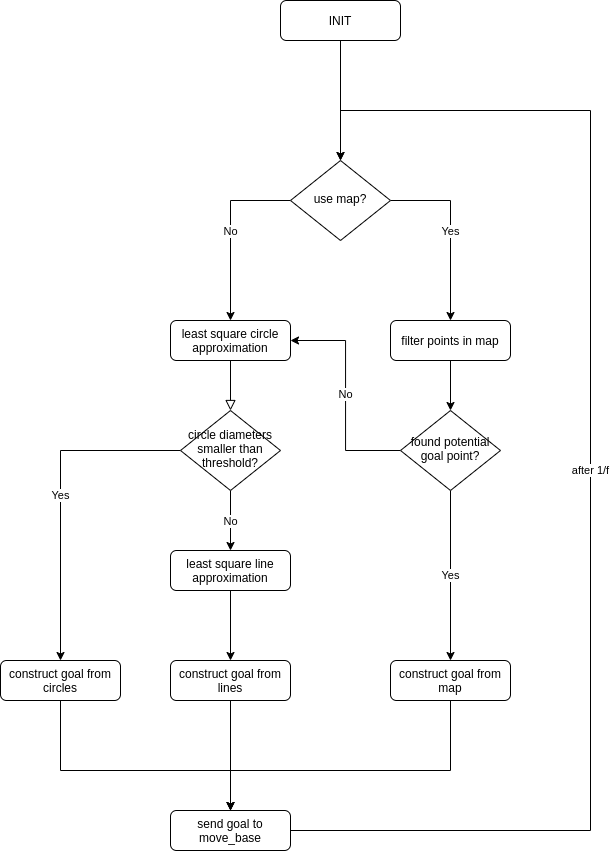
\includegraphics[width=.9\textwidth]{Pictures/posefinder diagram}
	\caption{Posefinder internal structure}
	\label{posefinder structure}
\end{figure}

The goalfinding algorithms are ordered in a hierarchic structure based on their expected accuracy.

A accurate map of the surrounding offers the best potential to find feasible goals on the upcoming road, hence it has to be checked first, if a goal can or should be extracted from the map.

Since as described every, even straight sections can be expressed by a circle segment, this approximation will have a higher priority than the line approximation.

Finally the line approximation will be checked last and only if the circle approximation generated circles with radii, that exceed a threshold for their trustworthiness.

The result of the chosen algorithm can be used to determine a goal that will be sent as an input to move\_base.

The node is configurable using rqt\_reconfigure and the following parameters.

\begin{table}[H]
\centering
\resizebox{\columnwidth}{!}{%
\begin{tabular}{ l l l }
	
 \textbf{Parameter} & \textbf{Description} & \textbf{Range}\\
 CRadThresh & The Threshold for the radius of the circle approximation & 0.5-20 [m]\\ 
 GoalDist & The maximum distance at which a goal should be found & 0.5-20 [m]\\  
 GoalAngle & The maximum angle for the circle approximation higher priority than distance & 0.1-2 [$\pi$]\\  
 reductionradius & Max Distance at which points from the map will still be combined & 0.25-2.5 [m]\\  
 MapCostThresh & Threshold Cost Value for Map Data Extraction & 0-100\\  

\end{tabular}
}

\caption{PoseFined parameters}
\label{posefinderparams}

\end{table}

\section{MarkFreeSpace}

Like described in the concept, the purpose of this node is to provide data to the SLAM algorithm as well as to the costmaps. This data consists from the points on the polynomials of the road detection in combination with the filtered points of the laser scan.\\

Based on the possibility of the obstacle\_layer of the costmap to raytrace marked obstacles, it needs to receive a PointCloud2 that contains points from the polynomials of the roadDetection. If this pointcloud would contain the points of the lidar aswell, the obstacle layer would remove the points of the road marking, if an obstacle is behind it.\\

For the slam algorithm both data sources need to be fused into one PointCloud2. Therefore the points need to be transformed into the same frame and into the same time, before being published.\\

The data of the dynamic cost layer has to contain more information. It is in the form of a sensor\_msgs::PointCloud and contains channel values for point individual inflation radius, min-cost and max-cost. By giving the layer point individual inflation parameters the node provides information about the cells on the left road marking that need to have inflated cost values and information about the points on the right road marking that should have a clear zone around them. Furthermore the node provides points of obstacles that are on the road and clears the inflated cost around it. This cleared zone makes the generation of path past the obstacle easier for the global planner.\\

The following parameters are offered for further configuration:

\begin{table}[H]
\centering
\resizebox{\columnwidth}{!}{%
\begin{tabular}{ l l l }
	
 \textbf{Parameter} & \textbf{Description} & \textbf{Range}\\
 MaxCost & Maximum cost of the left lane inflation & 0-254\\ 
 MinCost & Minimum cost of the left lane inflation & 0-254\\  
 LeftInflation & How far the inflation of the left lane overlaps the right lane & 0-1\\  
 RightRemoval & How much of the right lane will be cleared from cost & 0-1\\  
 ObstacleRemoval & Distance around obstacles on the road where no cost gets placed & 0-2 [m]\\  
 InflPointDistance & min Distance between inflated points 0 for only last & 0-5 [m]\\ 
 ClearPointDistance & min Distance between points that clear cost 0 for only last & 0-2 [m]\\   
\end{tabular}
}

\caption{MarkeFreeSpace parameters}
\label{markfreespaceparams}
\end{table}

\section{dynamic\_cost\_layer}
Enhancing to the plugins provided in the navigation stack this layer handles inflation of cells with a configurable cost decay and radius. While this seems to be similar to the provided inflation layer, this offers way more flexibility since it will inflate specific points by their individual radius and cost distribution and not just every lethal one by one fixed distribution.\\

This behavior can be used to inflate the left road marking in the global costmap to force the global plan on the right side of the road, which is the behavior defined in the concept. The plugin can also be used to inflate cells with zero cost, which is useful to guarantee a cost free right lane or to give some free space around obstacles located on the road.\\

The layer receives a message of type sensor\_msgs::PointCloud on a configurable topic. This point cloud is expected to feature channel values for the inflation radius, the maximal and the minimal cost for each individual point.\\

Since it can not be assumed, that the incoming points will be in the frame of the costmap the points in the costmap have to be transformed into the right frame using tf2.\\

To minimize the computation load a Bresenham based algorithm for the circle rasterization will be used\cite{ComputerGraphics}. Now the point symmetry around the cell can be used to further minimize the computational load and only $\frac{1}{8}$th of the circle has to be computed. The rasterization process can be described by the following image.\\

\begin{figure}
	\centering
	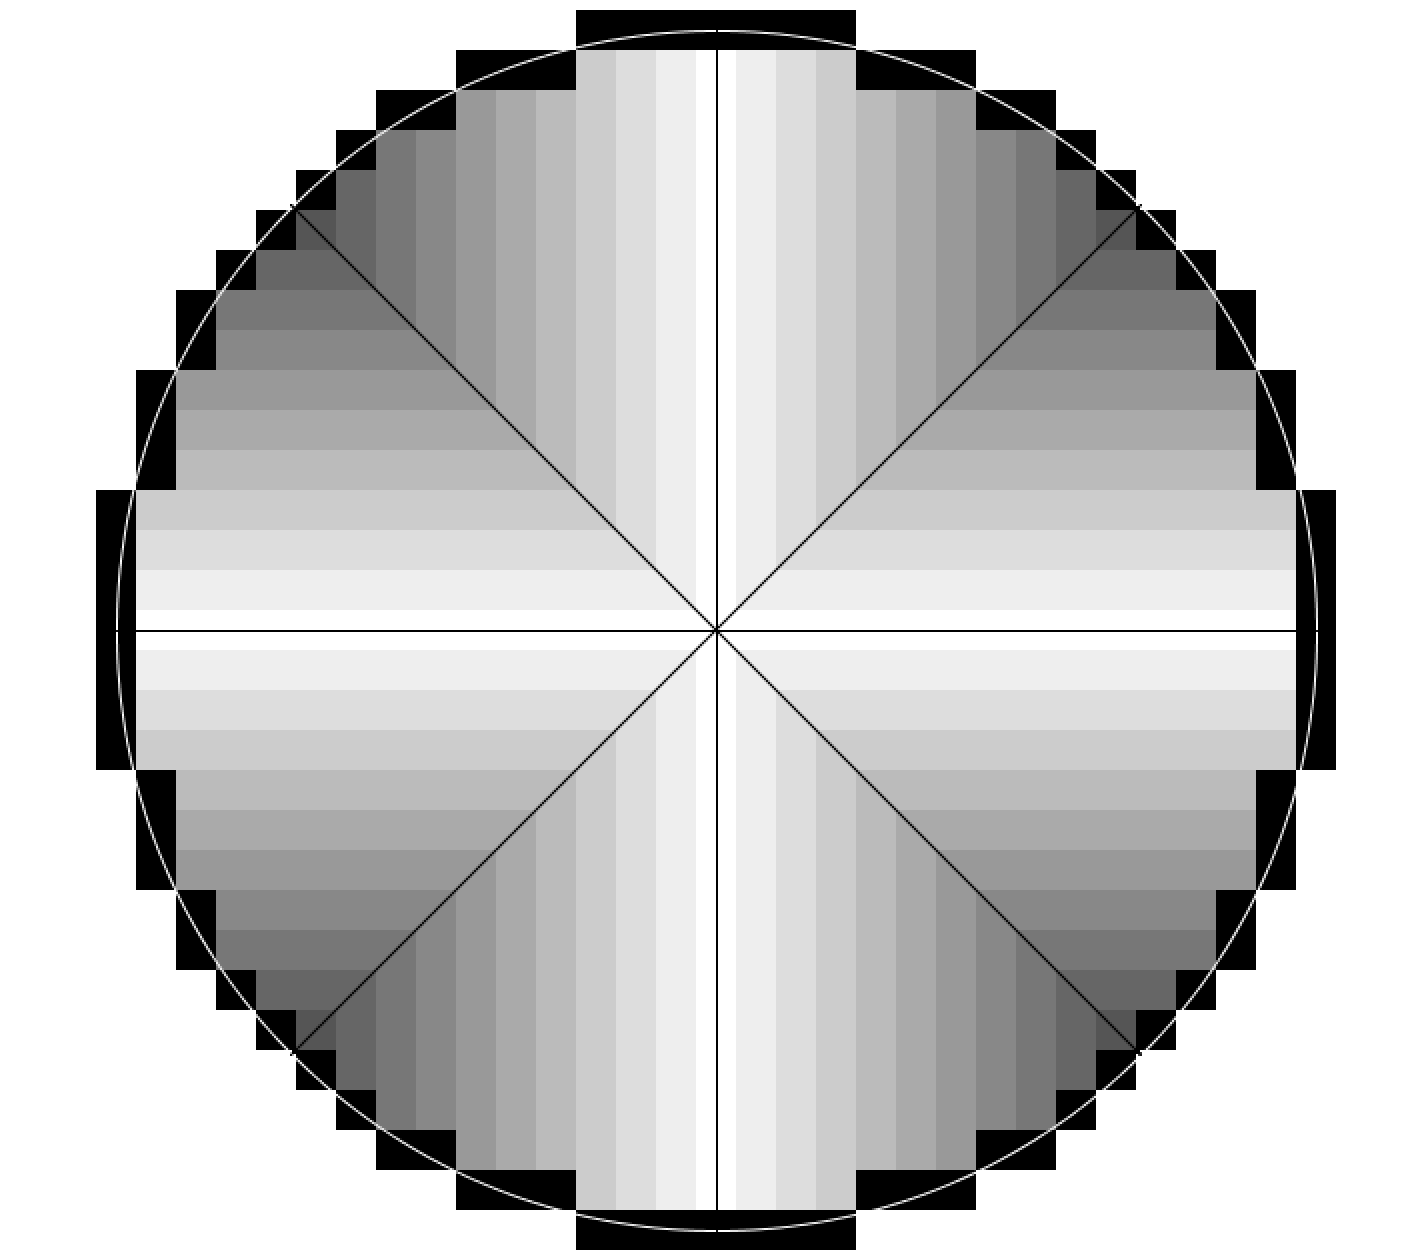
\includegraphics[width=.5\textwidth]{Pictures/rasterization}
	\caption{modified Bresenham rasterization with efficient surface filling}
	\label{rasterization}
\end{figure}


Adding to the typical behavior of the Bresenham rasterization the area of the circle will be filled using the point symmetry and by skipping overlapping points of the lines like in Figure \ref{rasterization}. Here it is visible, that every row with the same color is only calculated once and then projected in all eight octants. The black cells on the perimeter are the rasterized cells of the Bresenham algorithm.

The cells within the circles perimeter are filled with the cost specified for that point. For this the following linear decaying \nth{1} degree function will be used which requires the computation of the distance of the rasterized cell to the center of the circle.

\[cost(distance)=maxcost-distance*\frac{maxcost-mincost}{radius}\]\\
with: \[distance=\sqrt{cell.x^2+cell.y^2}\]

 Since this will still require the usage of a square root for each cell in the circle This will be optimized as well.\\

The goal here is to use a function that contains only the squared distance and not many other mathematical operators, which still represents a decaying trend. This requirement rules out every function with an odd degree, all functions with an x offset and the normal distribution. This leaves all functions with an even degree from which the \nth{2} degree function is chosen to reduce square operators. The comparison between the two functions can be seen in the picture below.

\[cost(distance)=maxcost-distance^2*\frac{maxcost-mincost}{radius^2}\]\\

\begin{figure}[H]
	\begin{center}
	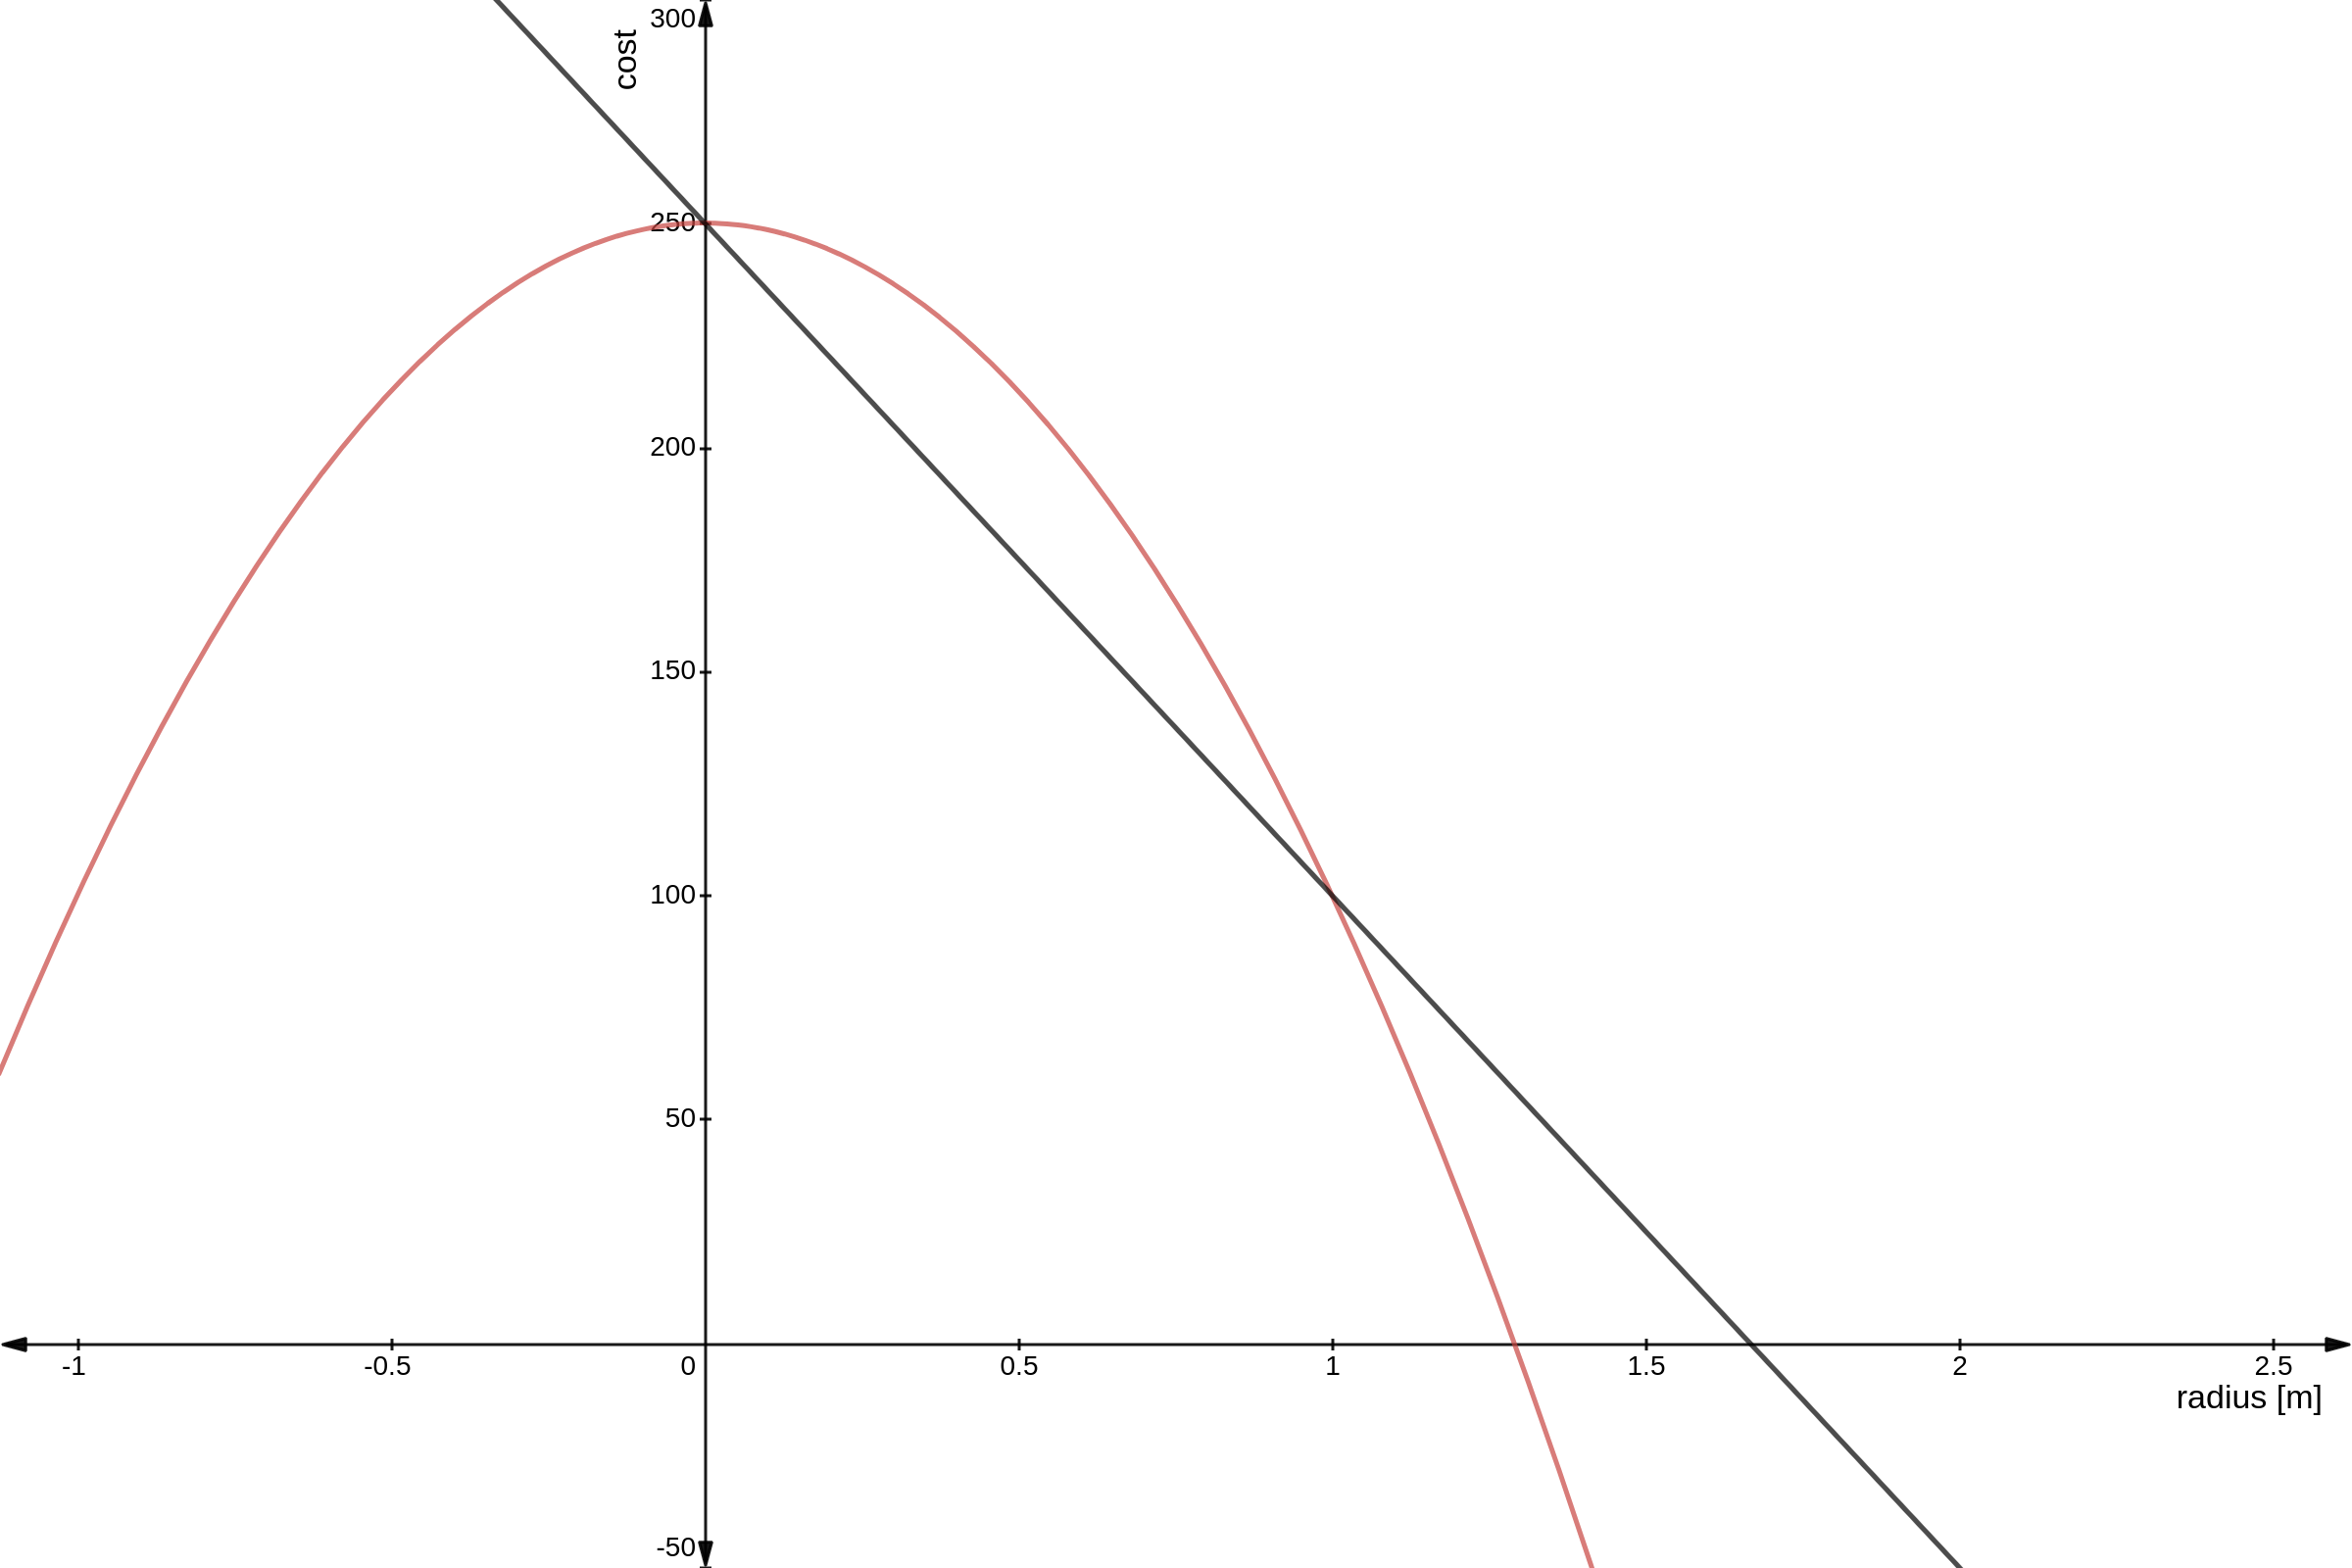
\includegraphics[width=140mm]{Pictures/linear cost comparison}
	\caption{cost distribution comparison with maxcost=250 mincost=100 radius=1}
	\end{center}
\end{figure}

The plugin can be configured individually for the costmap using rqt\_reconfigure and the following parameters.

\begin{table}[H]
\centering
\resizebox{\columnwidth}{!}{%
	\begin{tabular}{ l l l }
	
 	\textbf{Parameter} & \textbf{Description} & \textbf{Range}\\
 	enabled & Whether to apply this plugin or not & [bool]\\
 	point\_topic & The Topic of the PointCloud containing Points and channel values for inflation radius & [string]\\

	\end{tabular}
}
\label{dynlayerparams}
\caption{dynamic\_cost\_layer parameters}
\end{table}



\section{SLAM}
There are numerous lidar based SLAM packages available for ROS, but with the defined restriction of being able to use both, the points extracted from the road detection, as well as the lidar data, most of the lidar based SLAM algorithms wont work since they only accept one input of  the type sensor\_msgs::LaserScan.\\
This rules out the popular options for lidar based SLAM like gmapping and HectorSLAM and the well documented package Google Cartographer will be used based on its flexibility in regards to robot configurations.\\
This package comes with an advantage of being based on loop closure which might be useful when driving rounds in a circuit stile environment. The robot will drive the same route over and over again and thus the map could get more and more reliable over time even though the data is very self similar and not great for SLAM.\\

Cartographer accepts numerous different input types including both PointCloud2 and LaserScan sensor messages. Additionally Cartographer can use provided odometry, aswell as IMU data to improve the result.\\








